\documentclass[12pt]{article}

\usepackage{listings}
\lstset{
  language=Haskell
}

\usepackage{graphicx}
\graphicspath{ {../resources/haskell-emacs-workflow/} }

\usepackage[margin=1in]{geometry}

\usepackage[normalem]{ulem}

\usepackage[colorlinks]{hyperref}
\hypersetup{
  urlcolor = {cyan}
}

\title{A Beginner's Haskell Workflow in Emacs}
\author{Rushi Shah}
\date{5 December 2015}

\begin{document}

  \maketitle

What kind of programmer would I be if I didn't join the Vim vs.~Emacs
Crusades? Well I'm dabbling in Haskell, so emacs was the natural choice,
but I'm honestly not invested enough in either to speak to their
strengths or weaknesses.

However, regardless of your choice, it is a daunting task to use either
for the first time. Especially when learning a new language along with
it. So hopefully this post will demystify how to use Haskell with Emacs.

\section{Setup}\label{setup}

Honestly, I set up emacs and haskell and all a while ago, roughly
following
\href{https://github.com/serras/emacs-haskell-tutorial/blob/master/tutorial.md}{this
guide}. That in itself was an entire adventure, that I'm not even gonna
try to go through. All I will say is good luck, you \sout{might} will
need it.

\section{Opening a file and a Haskell
REPL}\label{opening-a-file-and-a-haskell-repl}

Aight, so down to business. First of all, in your plain old terminal,
navigate to the haskell file you're about to open. Let's assume it's
called
\href{https://github.com/2016rshah/adventofcode/blob/master/day2/Paper.hs}{Paper.hs}.

Start out by doing \texttt{emacs\ Paper.hs} to open the file. Make a few
edits or whatever until you're ready to start playing with functions in
GHCi. When you are, press \texttt{C-x-s} or \texttt{C-x\ C-s} to save
the file.

% \begin{figure}[htbp]
% \centering
% \includegraphics{\%7B\%7B\%20site.url\%20\%7D\%7Dblog/resources/emacs-haskell/two.png}
% \caption{File}
% \end{figure}
\begin{center}
\includegraphics[width=7in]{two}
\end{center}

Then press \texttt{C-c\ C-l} to start up an interactive Haskell REPL.
You will be prompted ``Start a new project named ``haskell''? (y or
n)'', so obviously answer with \texttt{y}. Press enter twice after that
for the two directories (I'm honestly not sure what they are both for)
and you will be greeted with a nice split screen between your file and
your interactive shell.

% \begin{figure}[htbp]
% \centering
% \includegraphics{\%7B\%7B\%20site.url\%20\%7D\%7Dblog/resources/emacs-haskell/three.png}
% \caption{File and terminal}
% \end{figure}
\begin{center}
\includegraphics[width=7in]{three}
\end{center}

\section{Terminal to file and back
again}\label{terminal-to-file-and-back-again}

Okay great, you've tested your functions and all, but you made a typo!
You need to go fix it in the file. But how do you get there?
\texttt{C-x\ o} (that's an o like octopus) will switch you back and
forth from the top and bottom buffers. When you are in the Haskell file,
you can press \texttt{C-c\ C-l} to load in the file. Or if you're
already in the REPL and don't want to switch over to the file to compile
it, you can just type in
\texttt{:l\ \textless{}FILE\_NAME\textgreater{}} to load it like normal
in GHCi.

\section{Opening more files}\label{opening-more-files}

Wait, you vaugely remember a sliver of syntax that you used in another
file yesterday, but you want to go check just to make sure. Navigate to
your haskell file if you're not already there. Then do \texttt{C-x-f} or
\texttt{C-x\ C-f} and find the path to the file you want to open. When
you press enter, it will overlay on the file you just had open. For
example, you want to go to
\href{https://github.com/2016rshah/adventofcode/blob/master/day2/Paper.hs}{Floor.hs}.
You found the syntax, its
\texttt{inp\ \textless{}-\ readFile\ "input.txt"}.

% \begin{figure}[htbp]
% \centering
% \includegraphics{\%7B\%7B\%20site.url\%20\%7D\%7Dblog/resources/emacs-haskell/four.png}
% \caption{New file}
% \end{figure}
\begin{center}
\includegraphics[width=7in]{four}
\end{center}

\section{Copy and Paste}\label{copy-and-paste}

But how are you going to remember it? By the time you switch back you
might remember it as getFile or readContents or any other permutation of
the wrong words. You need copy and paste. So first you need to select
the text you want to copy. To do so, go to the beginning of what you
need and press \texttt{C-@} (which is Ctrl, Shift, and 2 pressed all at
the same time on my keyboard). Then move your cursor to the end of what
you need. Press \texttt{M-w} to copy or \texttt{C-w} to cut. Just press
\texttt{C-y} to paste.

\section{Switching buffers}\label{switching-buffers}

But you don't want to paste here! You want to paste in the other file,
how do you get back to it? No need to open the file again with
\texttt{C-c\ C-f} because the buffer is already open. To switch back to
the previous buffer, do \texttt{C-x\ b} and you can probably press enter
because the default will be what you want. Did you accidentally type
\texttt{C-x\ C-b} and open a new buffer that you don't want with a list
of all the buffers? Switch over to it with \texttt{C-x\ o} and kill it
by pressing \texttt{C-x\ k} and pressing enter.

\section{Git}\label{git}

Okay so now you're all set up, you've solved your puzzle, but you want
to push your code to github! If you press \texttt{C-x\ C-c} to exit,
you'll have to open all your buffers again and it'll be a big mess. So
why not open up a shell within emacs over top of your Haskell REPL where
you can type in your git commands? Navigate to your REPL and press
\texttt{M-x}, then type in \texttt{shell}. Do your business with all the
git commands you know and love to commit/push your code. When your heart
is content, you can just press \texttt{C-x\ k} to kill the shell buffer
and continue on your merry way.

% \begin{figure}[htbp]
% \centering
% \includegraphics{\%7B\%7B\%20site.url\%20\%7D\%7Dblog/resources/emacs-haskell/five.png}
% \caption{Shell}
% \end{figure}
\begin{center}
\includegraphics[width=7in]{five}
\end{center}

\section{Other useful shortcuts}\label{other-useful-shortcuts}

\begin{itemize}
\item
  \texttt{C-n} to go to the \textbf{n}ext line
\item
  \texttt{C-p} to go to the \textbf{p}revios line
\item
  \texttt{C-f} to go \textbf{f}orward one character
\item
  \texttt{C-b} to go \textbf{b}ackwards one character
\item
  \texttt{C-g} to cancel any commands that are half-written when you
  realize you screwed up
\item
  \texttt{C-x\ u} to \textbf{u}ndo what you just did
\item
  \texttt{M-\textgreater{}} to jump to the end of the buffer
\item
  \texttt{M-p} to get the \textbf{p}revious command entered into the
  REPL. Similar to when you're in your terminal and you press the up
  arrow.
\item
  \texttt{M-x\ comment-region} after code is highlighted to comment it,
  \texttt{M-x\ uncomment-region} to uncomment.
\item
  \texttt{C-e} to jump to the \textbf{e}nd of the line
\item
  \texttt{M-g\ g} to jump to a specific line number
\item
  \texttt{C-x z} to redo the last command, and \texttt{z} to redo it again
  repeatedly (example: use after \texttt{C-x \^})
\item
  \texttt{C-x \^} to expand the size of the split screen that you're on
  by one line
\end{itemize}

\end{document}
